% Look Sebastian fisher (a play on regular expression) 
%   Really goes all the way 

% Student Sven is working on a Robot programming DSL supervised by Prof. Kurt. 
% Sven is beginner Haskeller
% Kurt is knowledgible (experienced)

% Introduction (Presents problem) 
%  Robot language operations. 
%  Robot exists that run programs in a simple language.
%  want to run code in robot. 
%  Haskell DSL and Do notation 
%  Compilation necessary.  

% Student has Haskell School of expression 
%   But need reifyable robot programs (evaluation not enough) 

% Show example program early 
%   Sven is a good student and early expresses an example program in his thought 
%   out API.
% 

% How to be able to use Do notation 
%  Adds Return and Bind naively to data structure. 

% Student brings --CODE SNIPPET-- to Prof. Kurt.

% Now the problem, how can this work? 
%  Prof. is familiar with Gills blog post. 

% Student brings --CODE SNIPPET-- (the compiler) to Prof. 


% Surprise 
% Work on generalisations  and make the compositionality explicit
% 

% What about the monad laws ? 
%  Prof. asks student to verify that Monad laws hold.


\subsection{Introduction}
\studname{} is a computer science student working in a project involving programming 
robots in a low-level imperative language. However, \studname{} has a budding 
interest in functional programming using Haskell and has read ``The Haskell 
school of expression'' \citebb{HUDAK}. He gets the idea to implement 
a language for robot control embedded in Haskell. \studname{} realises that the 
capabilities of the robot hardware are very similar to those of the 
robots that Hudak evaluates graphically in a grid world. There is however 
a very important difference; the embedded language needs to be compiled into 
some form that is understood by the robot. 
%\studname{} in a computer science student with a budding interest in functional 
%programming using Haskell. \studname{} is developing  
%an embedded domain specific language (EDSL) for robot control. Inspired 
%by the book ``the Haskell school of expression'' \citebb{HUDAK} but instead of 
%evaluating his robot EDSL, \studname{} wants to compile the language to a form 
%he can run on actual robot hardware. 
%with 
%different motivations, \studname{} wants compile his EDSL for actual physical robots, 
%he sets out. 

Guided by the capabilities of the target robot, \studname{} designs an API for 
robot programming. The robot can perform operations 
such as {\em move} that steps the robot forward and {\em turn} left and right. 
The robot also has the capability to execute program loops and conditionals and 
it has a forward facing {\tt sensor} with which it can query the world.

%The robot also has a forward facing {\tt sensor} with which it can query the 
%world and also the capabilities to execute program loops and conditionals. 
\pagebreak
The API that \studname{} designs is simple: 

%\begin{figure} 
\begin{small}
\begin{verbatim} 
move      :: Program () 
turnLeft  :: Program () 
turnRight :: Program ()
sensor    :: Program Bool 
cond      :: Program Bool 
             -> Program () 
             -> Program () 
             -> Program () 
while     :: Program Bool 
             -> Program () 
             -> Program () 
\end{verbatim}
\end{small} 
%\label{fig:interface} 
%\caption{Proposed set of basic robot operations}
%\end{figure}  

Now, \studname{} wants to express robot programs using the Haskell
{\em do} notation. The motivation behind this is the imperative look
and feel of the operations he identified and the potential to use all
the control structures in the {\em Control.Monad} library. For this, a
{\tt Monad} instance is needed.

To be able to create a first-order representation of a computation
described using monads, \studname{} needs to solve the problem of {\em
  reifying} monads. This is the story of how \studname{} came up with
a particularly simple solution to this problem.

%\emph{*** Josef, Think about writing here}

%\begin{minipage}[]{\linewidth}
%\vspace{5mm}

%\fbox{%
%\parbox{0.8\linewidth}{What \studname{} does not know at this time is that he has stumbled over the 
%problem of {\em Monad reification}. Monad reification is the observing of the shape of the computation and this is necessary in order to compile to some low level representation.}
%}
%\end{minipage}

\subsubsection{Example programs}

\studname{} is quite happy with his language design and decides to
write some programs to try it out.
%experiments 
%with what some of these robot controlling programs could look like once his 
%EDSL is finished. 

The first program is called {\tt sMove}, which implements a safe move 
operation. This operation can be executed by the robot even though it is facing 
an obstacle, without risk of harming robot or obstacle. 
%.It feels like a good idea to \studname{} to check the sensor before trying to 
%move the robot forward. Otherwise something in either the world or the 
%robot might suffer damage. 

\begin{small} 
\begin{verbatim}
sMove :: Program () 
sMove = cond sensor turnRight move 
\end{verbatim}
\end{small}  

The second program moves the robot forward until it stands directly 
in front of an obstacle such as a wall. 

\begin{small} 
\begin{verbatim}
moveToWall :: Program () 
moveToWall = while ((liftM not) sensor) move
\end{verbatim}
\end{small}  

Based on these examples, \studname{} is quite satisfied with the design of his
language and turns to implementing it.

\subsubsection{Implementation and data structures} 

Enthused by the prospect of compiling these programs to the target language and 
seeing some robot action, \studname{} goes to work on the data structures. 

% Since an abstract syntax representation of the robot programs is desired,
Since the language is going to be compiled, \studname{} realises that the 
booleans in his language cannot be regular Haskell booleans. The booleans 
needs to be replaced by boolean typed expressions.

\pagebreak
\begin{small} 
\begin{verbatim}
type Name = String

data BoolE = Lit Bool
           | Var Name
           | (:||:) BoolE BoolE
           | (:&&:)  BoolE BoolE
           | Not BoolE  
\end{verbatim} 
\end{small}  

Following this, the  operations that should go into the {\tt Program} data type 
feel straightforward.

\begin{small} 
\begin{verbatim}
data Program a where 
  Move      :: Program () 
  TurnLeft  :: Program () 
  TurnRight :: Program () 
  Sensor    :: Program BoolE
  Cond      :: Program BoolE 
               -> Program () 
               -> Program () 
  While     :: Program BoolE 
               -> Program () 
               -> Program () 
\end{verbatim} 
\end{small} 

\studname{} continues by naively adding constructors for {\tt Return} and 
{\tt Bind} to the {\tt Program} data type.   

\begin{small} 
\begin{verbatim}
data Program a where 
  ...
  Return :: a -> Program a 
  Bind   :: Program a 
            -> (a -> Program b)
            -> Program b 
\end{verbatim} 
\end{small} 

Then he writes down the {\tt Monad} instance.
 
\begin{small} 
\begin{verbatim}
instance Monad Program where 
  return = Return 
  (>>=)  = Bind 
\end{verbatim} 
\end{small} 

Proud of his accomplishments, \studname{} sends his Haskell module in an 
email to Prof. \docname{}. \studname{} knows that \docname{} is teaching an 
introductory Haskell course and should be able to provide feedback.



\subsubsection{Problem statement} 
\emph{Meanwhile in Professor \docname{}'s Office}\newline %\newline

\noindent Prof. \docname{} notices an email from \studname{} in his inbox and 
opens it. 

\vspace{5mm} 

\noindent\colorbox{light-gray}{
\begin{minipage}[]{0.9\linewidth}
\noindent 
Dear Professor \docname{}
\newline \newline
\noindent I am CS student working in a robot control project. Usually, we 
program our robots in C but I have developed an interest in Haskell 
programming and thought it'd be natural to try implementing an EDSL. 
I know you teach an FP course and thought I would ask for your input. 
Attached to this mail is a file containing an outline of the data types I 
want to use. Does this look sensible to you? \newline \newline

\noindent Thank you \newline
\noindent \studname{}
\end{minipage} 
}

%I have progressed some towards a robot programming language. Attached 
%to this mail is a first sketch of a {\tt Program a} data type for robot 
%programs.
\vspace{5mm}

Prof. \docname{} opens the attachment and takes a look at the data type. He 
particularly notices the constructors {\tt Return} and {\tt Bind} and the 
{\tt Monad} instance. He shakes his head at \studname{}'s naivet\'e and writes an 
email back:

%\vspace{5mm}

\noindent\colorbox{light-gray}{
\begin{minipage}[]{0.9\linewidth}
\noindent 
Hello \studname{}
\newline \newline
\noindent I'm afraid your implementation of the monadic primitives can never 
work. The constructor {\tt Return} can take any arbitrary value that has 
nothing to do with the language you're designing. These values may be 
strings, binary trees or higher-order functions from zygomorphisms to 
histomorphisms. The same problem goes for {\tt Bind}; it has to be able 
to handle arbitrary values. It cannot possibly work! This is a very 
difficult problem and such a naive solution is bound to fail. 
\newline \newline
%% \noindent For hints towards a solution to this I suggest that you follow 
%% this \underline{link} \citebb{GillBlog}. Another idea is that you refer 
%% to the article ``Generic monadic constructs for embedded languages'' 
%% \citebb{Generic}.
%% \newline \newline

\noindent Prof. \docname{} \newline
\noindent Dept. of Computer Science and Engineering \newline
\noindent Chalmers University of Technology 
\end{minipage} 
}

\vspace{5mm}


% \section{Implementation continues}
% \emph{Back to \studname{}'s implementation efforts} \newline \newline

\noindent While waiting for feedback from \docname{}, \studname{} has 
carried on trying to implement a compiler for his language. 

When \docname{}'s email does arrive, \studname{} is confused. He feels he 
has already managed to compile the {\tt Program} data type into a 
representation closer to that which is executed by the robot hardware. 

He writes an apprehensive email back to Prof. \docname{}. 

\vspace{5mm}

\noindent\colorbox{light-gray}{
\begin{minipage}[]{0.9\linewidth}
\noindent 
Hello Prof. \docname{} 
\newline \newline
\noindent Thanks for your feedback. But I think it does work! Attached
to this email you find a file containing my attempt at compiling the
{\tt Program} data type into a representation closer to that which is
executed by our robots. \newline \newline


\noindent I have also attached two example programs that you can compile and 
then run in the graphical simulator (see figure~\ref{fig:programs}) \newline \newline
%\vspace{5mm}

%\includegraphics[width=.49\linewidth]{./spiral1}
%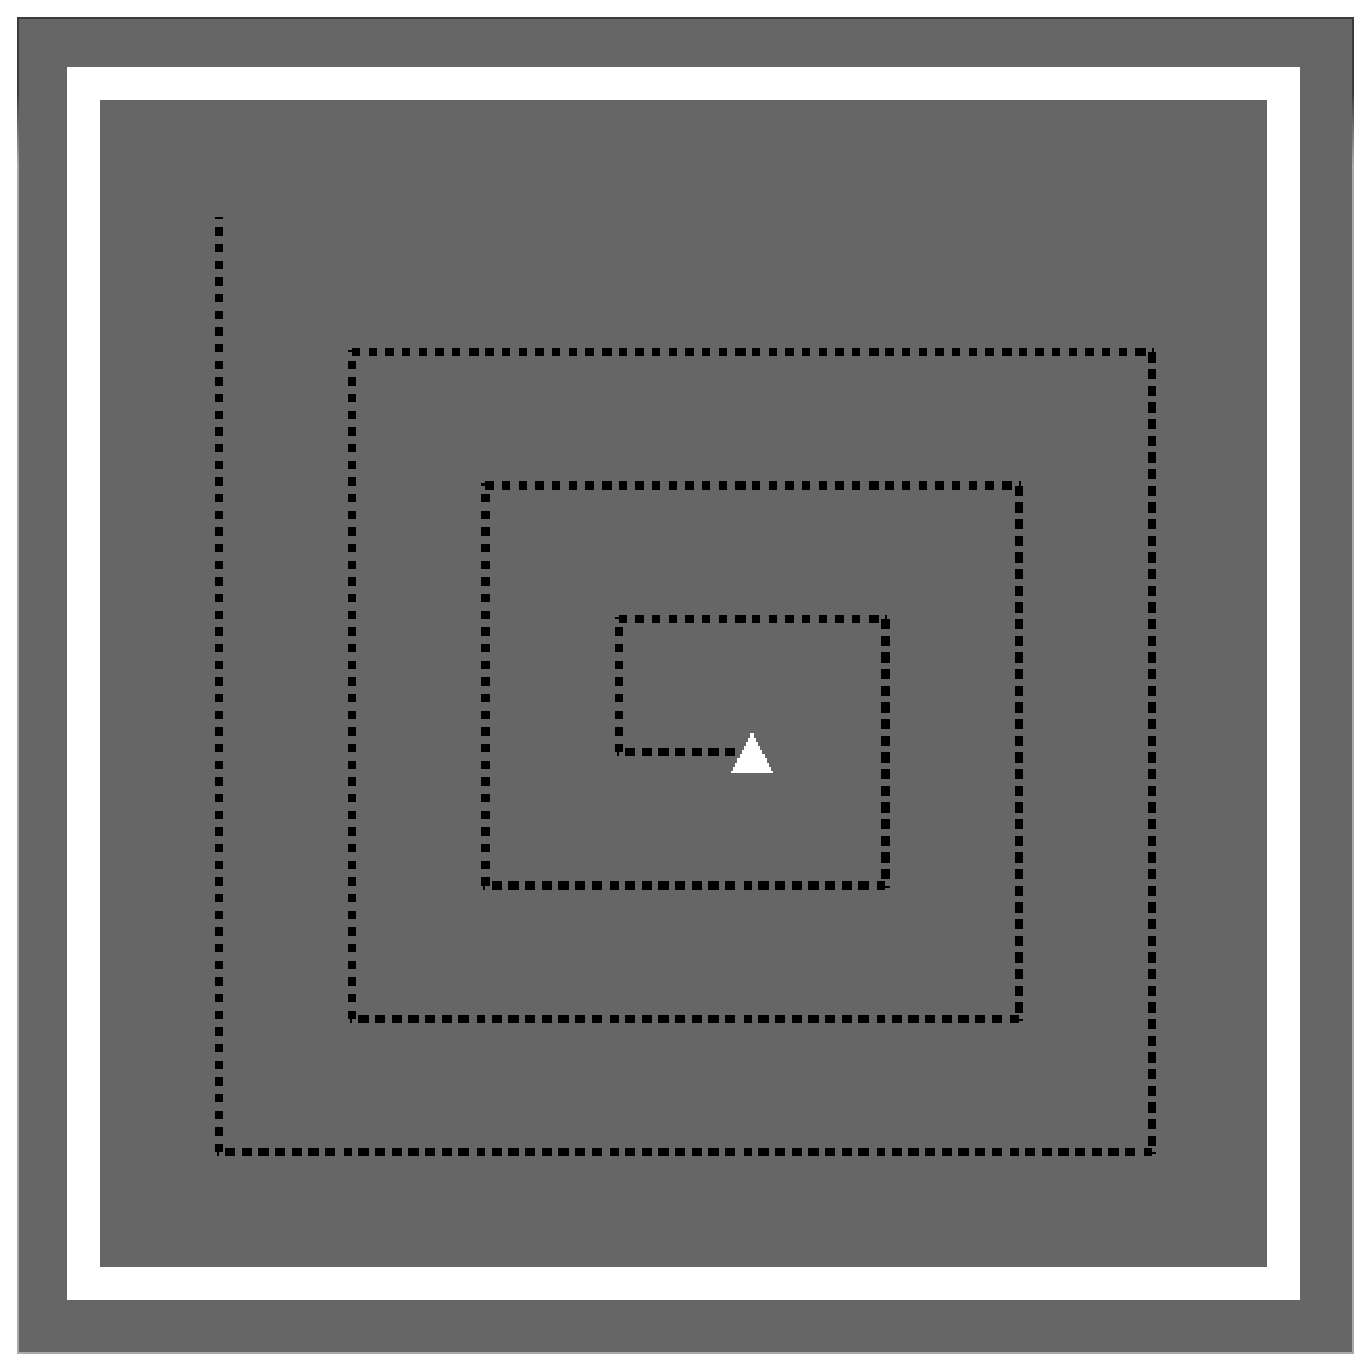
\includegraphics[width=.49\linewidth]{./spiral2}

%\vspace{5mm}

%\noindent And these two images are output from running the 
%{\tt followWall} (see figure~\ref{fig:followWall}) program. \newline

%\vspace{5mm}

%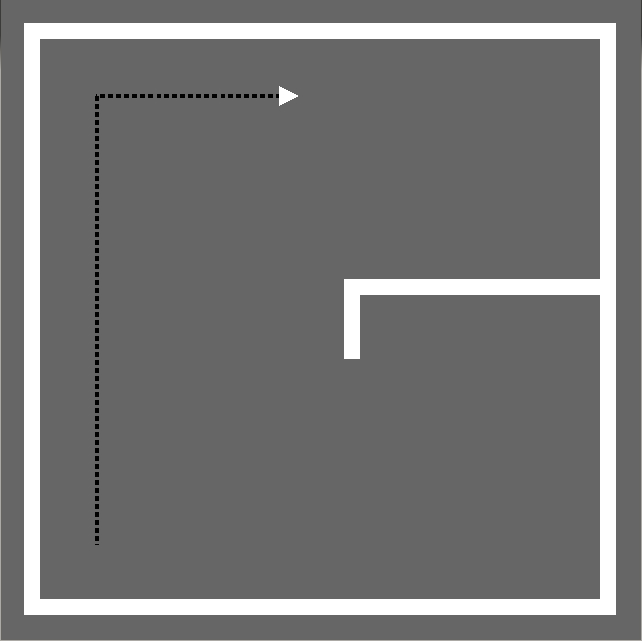
\includegraphics[width=.49\linewidth]{./wall1}
%\includegraphics[width=.49\linewidth]{./wall2}

%\vspace{5mm}

\noindent \studname{} 
\end{minipage} 
}

\FloatBarrier

\begin{figure*}
%\begin{tabular}{c|c}
\begin{minipage}[]{0.50\linewidth}
\begin{small}
\begin{verbatim}
spiralIn :: Int -> Program () 
spiralIn 0 = return () 
spiralIn n = do
  replicateM_ 2 $ do
    replicateM_ n move
    turnLeft
  spiralIn (n-1) 
\end{verbatim}
\end{small}
\end{minipage}
\hspace{0.05\linewidth} 
\begin{minipage}[]{0.45\linewidth}
\includegraphics[width=\linewidth]{./bb/spiral1}
\end{minipage}
%&
\begin{minipage}[]{0.50\linewidth}
\begin{small}
\begin{verbatim} 
followWall :: Program () 
followWall = 
  while (return true) $ 
    cond checkLeft sMove $ 
            do turnLeft
               move 

checkLeft :: Program BoolE     
checkLeft = do
  TurnLeft
  s <- Sensor
  TurnRight 
  return s
\end{verbatim}
\end{small}
\end{minipage}
\hspace{0.05\linewidth}
\begin{minipage}[]{0.45\linewidth}
\includegraphics[width=\linewidth]{./bb/wall2}
\end{minipage}

%\end{tabular}
\caption{The {\tt spiralIn} and {\tt followWall} programs sent from \studname{}
to \docname{} in an email}
\label{fig:programs}
\end{figure*} 



\subsection{Compilation of the monadic robot EDSL} 
\emph{\docname{} receives \studname{}'s latest email}\newline %\newline 

\noindent \docname{} looks through the {\tt Compiler} module and finds a data type describing
a first-order representation of the robot language.

\begin{small} 
\begin{verbatim}
data Prg = PMove          
         | PTurnRight
         | PTurnLeft
         | PSensor Name  
         | PCond BoolE Prg Prg
         | PWhile Name Prg Prg 
         | PSeq Prg Prg
         | PSkip       
         | PAssign Name BoolE
\end{verbatim}
\end{small}

\begin{figure} 
\begin{small}
\begin{verbatim} 
newNameSupply :: NameSupply 
split2 :: NameSupply -> 
          (NameSupply,NameSupply) 
split3 :: NameSupply -> 
          (NameSupply,NameSupply,NameSupply)
supplyValue :: NameSupply -> Int 
\end{verbatim} 
\end{small}
\caption{The interface of the splittable name supply used in the implementation 
of the compile functions} 
\label{fig:namesupply}
\end{figure}

From the {\tt Prg} data type, \docname{} presumes that the {\tt PSeq}
constructor will be the result of compiling {\tt Bind} and that
{\tt PSensor} binds a variable which can be used in {\tt PAssign} and
{\tt PWhile}. The conclusion is that the representation looks
sensible, but he is very interested in seeing the {\tt Program a -> Prg}
transformation. The compile function assumes a splittable name
supply with the interface described in figure \ref{fig:namesupply}.

%\pagebreak
\begin{small} 
\begin{verbatim}
runCompile :: Program a -> Prg
runCompile prg = snd $ compile s prg 
  where 
    s = newNameSupply
    
compile :: NameSupply -> Program a -> (a, Prg) 
compile s Move = ((),PMove)
compile s TurnRight = ((),PTurnRight)
compile s TurnLeft  = ((),PTurnLeft)
compile s Sensor    = (Var nom,PSensor nom)
  where
    v   = supplyValue s
    nom = "v" ++ show v 
compile s (Cond b p1 p2) = 
    ((),bp `PSeq` PCond b' p1' p2') 
  where
    (s1,s2,s3) = split3 s
    (b',bp)    = compile s1 b
    (a1,p1')   = compile s2 p1
    (a2,p2')   = compile s3 p2
compile s (While wp prg) = ((),PWhile nom nwp prg') 
  where
    (s1,s2,s3) = split3 s
    (b,wp')    = compile s1 wp
    (c,prg')   = compile s2 prg 
    nom        = "v" ++ (show $ supplyValue s3)
    nwp        = (wp' `PSeq` PAssign nom b) 
compile s (Return a) = (a,PSkip)
compile s (Bind pa f) = (b, prg1 `PSeq` prg2) 
  where
    (s1,s2)  = split2 s
    (a,prg1) = compile s1 pa
    (b,prg2) = compile s2 (f a) 
\end{verbatim}
\end{small}

%\begin{small} 
%\begin{verbatim}
%compile :: Program a -> Prg
%compile prg = snd $ compile' s prg 
%  where 
%    s = unsafePerformIO $ newEnumSupply
%    
%compile' :: Supply Int -> Program a -> (a, Prg) 
%compile' s Move = ((),PMove)
%compile' s TurnRight = ((),PTurnRight)
%compile' s TurnLeft  = ((),PTurnLeft)
%compile' s Sensor    = (Var nom,PSensor nom)
%  where
%    v = supplyValue s
%    nom = "v" ++ show v 
%compile' s (Cond b p1 p2) = ((), PCond b p1' p2') 
%  where
%    (s1,s2) = split2 s
%    (a1,p1') = compile' s1 p1
%    (a2,p2') = compile' s2 p2 
%compile' s (While wp prg) = ((),PWhile nom nwp prg') 
%  where
%    (s1,s2,s3) = split3 s
%    (b,wp') = compile' s1 wp
%    (c,prg') = compile' s2 prg 
%    nom  = "v" ++ (show $ supplyValue s3)
%    nwp = (wp' `PSeq` PAssign nom b) 
%compile' s (Return a) = (a,PSkip)
%compile' s (Bind pa f) = (b, prg1 `PSeq` prg2) 
%  where
%    (s1,s2) = split2 s
%    (a,prg1) = compile' s1 pa
%    (b,prg2) = compile' s2 (f a) 
%\end{verbatim}
%\end{small}

\docname{} studies the code in disbelief, saves the module and tries
it out on some examples. The code does indeed seem to work and
\docname{}'s disbelief is replaced with enthusiasm; this appears to be
a simple and convenient way to reify monads.
%What's more it does so in a 
%compositional way. The compilation of the {\tt Return} and {\tt Bind} cases 
%are completely independent of any other construct of the language. 

\docname{} sends an email to \studname{}, inviting him to a meeting. 

\subsection{Meeting in \docname{}'s office} %\section{Related Work} 
%\emph{Meeting in \docname{}'s office} \newline 

%TODO Here I want to cast light on more related work 
%and have \docname{} and \studname{} compare their approach to some of the existing ones. 
%also they should start sketching out the Idea of using {\tt CompData} instead 
%of a la carte for showing the compositionality. 

%\begin{minipage}[]{\linewidth}
\begin{dialogue} 

\speak{\docname{}} Hello, come in. 

\speak{\studname{}} Thanks. 

\speak{\docname{}} So, about this robot language! You gave me a bit of a 
surprise there. I was entirely sure that what you did was impossible. 

\speak{\studname{}} Oh, But I just did the first thing that came to mind. 
There was no deep thought behind it. 

\speak{\docname{}} The problem is \direct{\docname{} approaches his whiteboard}
 when you try to reify the bind constructor of your representation.
\end{dialogue} 


%\mbox{ 
\begin{small}
\begin{Verbatim}[commandchars=\\\{\}] 
Bind :: Program a -> \underline{(a -> Program b)} -> Program b 
\end{Verbatim}
\end{small}
%}


\begin{dialogue}
\speak{\docname{}} You need to come up with an element of type {\tt a} to 
pass to the function. 

\speak{\studname{}} I didn't realise it was problem. 

\speak{\docname{}} But it is! Your solution is that you are careful
about the return types of all operations in your language. They are
either of unit type or some type which can be guaranteed to be reified.
\direct{\docname{} scribbles on his whiteboard}

\end {dialogue} 

\begin{small}
\begin{Verbatim}[commandchars=\\\{\}] 
Move :: Program \underline{()}
  
Sensor :: Program \underline{BoolE}
\end{Verbatim}
\end{small}

\begin{dialogue}
\speak{\docname{}} This is different from how such constructs are
normally implemented. If I had implemented the language I would have
given {\tt Sensor} the type {\tt Program Bool} so that I could write
an evaluator of type {\tt Program a -> a}, or perhaps {\tt Program a -> M a}.
But then adding a monad to the language and reifying it becomes much harder.

\speak{\studname{}} Yes, now that you mention it, I have seen that style used
for defining DSLs.

\speak{\docname{}} Having constructors like {\tt Sensor} return {\tt
  BoolE} instead of {\tt Bool} is a crucial part of why your
method works. It allows the {\tt compile} function to be written in
such a way that it can generate the return values statically and pass
them as arguments to {\tt Bind}. In a sense you're doing evaluation at
the same time as compilation. There's just enough evaluation to
remove the monadic constructs. It's a very neat trick!

\speak{\studname{}} Thank you.

\speak{\docname{}} Another way to think about your trick is that you are
using a writer monad to evaluate your language and produce the first-order
syntax tree as a side effect. Then you could have used a state monad
transformer on top of that for the fresh name supply. But that's a stylistic
choice.

\speak{\studname{}} You seem to be making a big deal out of this. I
just did what I thought was the most straightforward thing to do.

\end{dialogue}

\subsubsection{Related work} 

\begin{dialogue}

\speak{\docname{}} Others have solved this problem before but I have
never seen a solution as simple as yours and was quite surprised that
it works. For example, in this paper \direct{\docname{} shows
  \studname{} the paper \citebb{Generic}}, the authors use a
continuation monad to be able to reify the monadic constructs of their
language. If they were to implement your robot language they would use
the same \texttt{Program} data type as you do. However, they would not
expose that to the user of the language. Instead they would create a
type like this:

\end{dialogue}

\begin{small}
\begin{verbatim}
data P a =
  P (forall r. ((a -> Program r) -> Program r))
\end{verbatim}
\end{small}

\begin{dialogue}
\speak{\docname{}} The type \texttt{P} is a continuation monad so the
monad instance comes naturally. Operations on \texttt{P} are defined
using \texttt{Bind} like this:
\end{dialogue}

\begin{small}
\begin{verbatim}
while :: P BoolE -> P () -> P ()
while c b =
  P (\k -> While (runP c) (runP b) `Bind` k)
\end{verbatim}
\end{small}
%\pagebreak
\begin{small}
\begin{verbatim}
cond :: BoolE -> P () -> P () -> P ()
cond b t e =
  P (\k -> Cond b (runP t) (runP e) `Bind` k)

runP :: P a -> Program a
runP (P f) = f (\a -> Return a)
\end{verbatim}
\end{small}

\begin{dialogue}
\speak{\studname{}} I see. Continuations are quite magical to me. I
could never have come up with that technique. How do they deal with
transforming higher-order programs to first-order programs?

\speak{\docname{}} That's a good question. The transformation to first
order programs is dealt with by a library called Syntactic. It is
described in a separate paper \direct{\docname{} pulls out the paper
  \citebb{SyntacticICFP12} from a pile of papers}. It's hard to do
an apples to apples comparison between Syntactic and your
technique. Syntactic solves a much bigger problem than what you're
doing so it is naturally more complicated.

\speak{\studname{}} Ok.

\speak{\docname{}} There are also the papers
\citebb{Farmer,sculthorpe2013constrained} which solves
the problem in a manner that is more similar to yours. They also have explicit
constructors {\tt Bind} and {\tt Return} but give them a slightly different
type which guarantees that all applications of {\tt Bind} are {\em normalised},
so that all {\tt Bind}s are right-associated. Unexpectedly, this
allows them to make instances of the {\tt Monad} class but at the same time
constrain the arguments of {\tt Bind}.
Their technique is more complicated than yours, but just as with the
case of Syntactic, they solve a more general problem.

However, there is one particular thing I like about your technique.

\speak{\studname{}} What is that?

\speak{\docname{}} Your technique is compositional.

\end{dialogue}

\subsubsection{Compositionality} 

\begin{dialogue} 
\speak{\studname{}} What does it mean that my technique is compositional?

\speak{\docname{}} The compile function is compositional because there
is one case for each constructor and each case deals with exactly one
constructor. In particular, the constructors {\tt Return} and {\tt
  Bind} are handled completely separately from all other language
constructs.

\speak{\studname{}} And that is good ? 

\speak{\docname{}} Absolutely! Compositional definitions are nice
because they imply that there is no weird semantical interaction
between the constructs as they are defined independently. But it also
means that it should be possible to factor out the constructors
\texttt{Return} and \texttt{Bind} into a data type of their own. Then,
it could be combined with other data types using techniques like Data
Types \'{a} la Carte \citebb{Wouter} or CompData \citebb{CompData}. This
way, a language can be designed piece by piece.You can then select the
set of pieces required for a particular task or that suits a
particular brand of robots.

\speak{\studname{}} Oh! Interesting.
\end{dialogue}


\subsubsection{The Monad laws} 

\begin{dialogue}
\speak{\docname{}} There is still one problem with your method though.

\speak{\studname{}} What's that?

\speak{\docname{}} When we make instances of the monad class we expect
certain laws to hold. \direct{\docname{} writes the laws on his whiteboard}

\end{dialogue}

\begin{small}
\begin{verbatim}
m >>= return    = m
return a >>= f  = f a
(m >>= f) >>= g = m >>= \a -> f a >>= g
\end{verbatim}
\end{small}

\begin{dialogue}
\speak{\docname{}} These laws clearly don't hold for your instance. Take the
first law for instance. The left hand side will have extra \texttt{Bind} and
\texttt{Return} constructors compared to the right hand side.

\speak{\studname{}} Hmmm. I hadn't really thought about that. But adding an
extra return at the end of a computation shouldn't make a difference
in my implementation.

\speak{\docname{}} So, you're saying that your implementation actually obeys
the first monad law?

\speak{\studname{}} Well, at least when I run my programs I will never see
any difference between the left hand side and the right hand side.

\speak{\docname{}} Aha, so what you're saying is that if we compare the
semantics of programs rather than comparing the programs themselves
then we get some useful laws. \direct{\docname{} scribbles some new laws
  on the whiteboard}

\end{dialogue}
%\end{minipage}

\begin{small}
\begin{verbatim}
eval (m >>= return)    = eval m
eval (return a >>= f)  = eval (f a)
eval ((m >>= f) >>= g) = eval (m >>= \a -> f a >>= g)
\end{verbatim}
\end{small}

%\begin{minipage}[]{\linewidth}
\begin{dialogue}
\speak{\docname{}} These laws are morally the same as the monad
laws, especially if we don't let the user of the robot language ever
compare terms in the language.

\speak{\studname{}} Yes, that captures my intuition very well.

\speak{\docname{}} Ok, good. Can you prove these equations?

\speak{\studname{}} No, I don't have any experience proving programs correct.

\speak{\docname{}} Well, it shouldn't be that difficult. Let me see
what I can come up with.

\direct{\docname{} scribbles frenetically on a piece of paper for a
  couple of minutes.}

Aha! Your technique is quite general. It can reify
monads into any kind of structure which is a monoid. Return translates
into the monoid unit and bind translates into the monoid operation.

For example, in your compilation function it is important that the semantics of
\texttt{PSkip} is the identity of the semantics of \texttt{PSeq} and that
\texttt{PSeq}
is associative.
\speak{\studname{}} Ok, that sounds good. I take that as meaning the method
is quite general? 

\speak{\docname{}} Yes, requiring a monoid is a very mild restriction. 

Look at the time! This was interesting, I got quite carried away. We must 
round off but please get back to me if you make any more progress on your 
robot language.

\speak{\studname{}} Thanks very much for your time. Bye!
\speak{\docname{}} Thank you. 

\end{dialogue}

\subsection{Composing reifiable monadic languages} 
\label{sec:composing} 

\emph{At \studname{}'s computer} \newline

\studname{} was really intrigued by the idea of compositionally
building embedded languages and after having read the papers
\docname{} showed him he decides to try his own approach to the problem.

Inspired by CompData he starts out by adding the code in figure
\ref{fig:compdata} to his file. The data type \texttt{:+:} is used for
composing languages, and the \texttt{:<:} typeclass provides coercions
so that the programmer doesn't have to worry about using the right
sequence of the \texttt{InjL} and \texttt{InjR} constructors to inject
terms into the composed language.

\begin{figure}
\begin{small}
\begin{verbatim}
data (e1 :+: e2) x a 
  = InjL (e1 x a) | InjR (e2 x a)
infixr :+:

class sub :<: sup where
  inj :: sub x a  -> sup x a

instance f :<: f where
  inj = id

instance (f :<: (f :+: g)) where
   inj = InjL  

instance (f :<: h) => (f :<: (g :+: h)) where
  inj = InjR . inj 
\end{verbatim}
\end{small}
\caption{Data types from CompData for composing languages.}
\label{fig:compdata}
\end{figure}

\studname{} then starts to add data types for the different language
constructs in his robotic language. The different operations for the
robot are pleasingly easy to add.
%\pagebreak
\begin{small}
\begin{verbatim}
data MoveOp x a where 
  Move :: MoveOp x () 

data TurnOp x a where 
  TurnLeft  :: TurnOp x () 
  TurnRight :: TurnOp x () 

data SensorOp x a where 
  Sensor :: SensorOp x BoolE

data CondOp x a where 
  Cond :: x BoolE -> x () -> x () -> CondOp x () 

data WhileOp x a where 
  While :: x BoolE -> x () -> WhileOp x () 
\end{verbatim}
\end{small}

In order to test out these definitions, \studname{} next turns to
implementing a compiler. He realises that the compiler now needs to be
implemented as a class with one instance per compilable sub-language.

\begin{small}
\begin{verbatim}
runCompile :: Compile f => f a -> Prg
runCompile prg = snd $ compile s prg
  where s = newNameSupply 

class Compile f where
  compile :: NameSupply -> f a -> (a, Prg)

instance Compile (MoveOp x) where
  compile _ Move = ((), PMove) 

instance Compile (TurnOp x) where
  compile _ TurnLeft = ((), PTurnLeft)
  compile _ TurnRight = ((), PTurnRight)

instance Compile (SensorOp x) where
  compile s Sensor = (Var nom, PSensor nom)
    where v   = supplyValue s
          nom = "v" ++ show v
\end{verbatim}
\pagebreak
\begin{verbatim}
instance Compile x => Compile (CondOp x) where
  compile s (Cond b p1 p2) = 
    ((),bp `PSeq` PCond b' p1' p2') 
    where (s1,s2,s3) = split3 s
          (b',bp)    = compile s1 b
          (a1,p1')   = compile s2 p1
          (a2,p2')   = compile s3 p2 
\end{verbatim}
\end{small}
%% instance Compile x => Compile (CondOp x) where
%%   compile s (Cond b p1 p2) = ((),PCond b p1' p2') 
%%     where
%%       (s1,s2) = split2 s
%%       (a1,p1') = compile s1 p1
%%       (a2,p2') = compile s2 p2 
%\pagebreak
\begin{small}
\begin{verbatim}
instance Compile x => Compile (WhileOp x) where
  compile s (While wp p) = ((),PWhile nom nwp p')
    where (s1,s2,s3) = split3 s
          (b,wp')    = compile s1 wp
          (c,p')     = compile s2 p
          nom        = "v" ++ (show $ supplyValue s3)
          nwp        = wp' `PSeq` PAssign nom b

instance (Compile (e1 f), Compile (e2 f)) 
  => Compile ((e1 :+: e2) f) where
  compile s (InjL a) = compile s a
  compile s (InjR a) = compile s a 
\end{verbatim}
\end{small}

But when \studname{} tries to add the monadic operations he finds that
they are quite resistant to a compositional treatment. After much
struggle he comes up with the following data type definition:

\begin{small}
\begin{verbatim}
data Mops f x a where
  Oper   :: f x a -> Mops f x a
  Return :: a -> Mops f x a
  Bind   :: x a -> (a -> x b) -> Mops f x b
\end{verbatim}
\end{small}

The recursion is provided by another data type that \studname{} 
calls {\tt MonadExp}.

\begin{small}
\begin{verbatim}
data MonadExp f a = In (Mops f (MonadExp f) a)
\end{verbatim}
\end{small}

\studname{} thinks of the {\tt MonadExp} data type as a representation
of a monadic language parameterised over operations {\tt Oper} that
are constructed using the constructors of some type {\tt f}. The monad
instance for this data type is only slightly more complicated compared
to the earlier, non-compositional setting.

\begin{small}
\begin{verbatim}
instance Monad (MonadExp f) where 
  return = In . Return
  (>>=) a f = In (Bind a f) 
\end{verbatim}
\end{small}

\studname{} can now write the type of his robotic language, built
from independent pieces. It is noteworthy that the monadic expressions
have to be added on top of all the other language constructs.

\begin{small}
\begin{verbatim}
type Robot = MonadExp (MoveOp :+: TurnOp  :+:
                       CondOp :+: WhileOp :+:
                       SensorOp)
\end{verbatim}
\end{small}

Given the definition of his language \studname{} can now write an
injection function which helps writing smart constructors for all the
different robot operations.

\begin{small}
\begin{verbatim}
inject :: (sub :<: f) 
       => sub (MonadExp f) a 
       -> MonadExp f a
inject a = In $ Oper $ inj $ a 

move :: (MoveOp :<: f) => MonadExp f ()
move =  inject Move 

turnL :: (TurnOp :<: f) => MonadExp f ()
turnL = inject TurnLeft

turnR :: (TurnOp :<: f) => MonadExp f ()
turnR = inject TurnRight

sensor :: (SensorOp :<: f) => MonadExp f BoolE
sensor = inject Sensor 
\end{verbatim}
\end{small}

\begin{small}
\begin{verbatim}
cond :: (CondOp :<: f) 
     => MonadExp f BoolE 
     -> MonadExp f () -> MonadExp f () -> MonadExp f ()
cond b p1 p2 = inject $ Cond b p1 p2

while :: (WhileOp :<: f) 
      => MonadExp f BoolE 
      -> MonadExp f () -> MonadExp f ()
while pb p = inject $ While pb p
\end{verbatim}
\end{small}

Things are starting to fall into place. The only remaining bit is to
complete the compiler for monadic expressions.

\begin{small}
\begin{verbatim}
instance (Compile x, Compile (f x)) 
  => Compile (Mops f x) where
  compile s (Oper o) = compile s o
  compile s (Return a) = (a,PSkip)
  compile s (Bind m f) = (b,prg1 `PSeq` prg2) 
    where (s1,s2)  = split2 s
          (a,prg1) = compile s1 m
          (b,prg2) = compile s2 (f a)

instance (Compile (f (MonadExp f))) 
  => Compile (MonadExp f) where
  compile s (In a) = compile s a
\end{verbatim}
\end{small}

Now, \studname{} has all the functions he needs to compile a simple
example program.

\begin{small}
\begin{verbatim}
test1 :: Robot () 
test1 = do 
  move
  turnL
  move 
  turnL 
\end{verbatim}
\end{small}

Compiling the program above gives the expected result. 

\begin{small}
\begin{verbatim}
PSeq PMove (PSeq PTurnLeft (PSeq PMove PTurnLeft))
\end{verbatim}
\end{small}


\studname{} decides to contact \docname{} again to show him what 
he has done.

\vspace{5mm}

\noindent\colorbox{light-gray}{
\begin{minipage}[]{0.9\linewidth}
\noindent 
Dear Prof. \docname{}
\newline \newline
\noindent I have attached a file which demonstrates that the monadic
constructs can be factored out and compiled separately, just as you
suggested.
\newline \newline

\noindent Thanks \newline
\noindent \studname{}
\end{minipage} 
}

\vspace{5mm} 

\noindent\colorbox{light-gray}{
\begin{minipage}[]{0.9\linewidth}
\noindent 
\studname{},
\newline

Fascinating! You've managed to factor out the monadic operations so
that they can be compiled once and for all. Users of your library
don't have to be concerned at all with the semantics of bind and return.
Very nice!
\newline
%% \end{minipage}}

%% \noindent\colorbox{light-gray}{
%% \begin{minipage}[]{0.9\linewidth}
\noindent 
I note that the data type for monadic operations cannot be composed as
freely as the other operations, but instead has to be applied
separately as a final step. Your
solution is very similar to how variable binding is handled in the
Syntactic library \citebb{syntactic}.
\newline \newline

\noindent Prof. \docname{}
\newline
\noindent Dept. of Computer Science and Engineering \newline
\noindent Chalmers University of Technology 
\end{minipage} 
}


%One of the advantages of the monad reification technique we have
%presented is that it is compositional. The monadic constructs can be
%dealt with separately from all the primitives of the embedded
%languages.

%A consequence of the compositionality is that we can use techniques
%such as CompData \citebb{} to decompose the definition of DSLs into
%smaller reusable building blocks. Figure \ref{fig:compdata} shows a
%compositional implementation of the monadic constructs, separately
%from any other constructs. The type \verb!Cxt! is defined in the
%package CompData and ties the recursive knot.

%\begin{figure}
%\begin{verbatim}
%data MonadT r a where
%  Return :: a -> MonadT r a
%  Bind   :: r a -> (a -> r b) -> MonadT r b

%instance (MonadT :<: f) => Monad (Cxt h f a) where
%  return a = iReturn a
%  m >>= f  = iBind m f
%\end{verbatim}
%\label{fig:compdata}
%\caption{Compositional definition monads}
%\end{figure}


%\end{minipage}

% \docname{} calls upon \studname{} to tally up the limitations of his approach 

% Monad Laws (Do the hold ?) 
% Infinite programs 
% Only certain ``kinds'' of reification!

\subsection{Epilogue} 

%This short story has outlined the discovery process and the many turns from 
%hopefulness to despair and back to hopefulness of two people who met over 
%a language embedded in Haskell. 
%% This was the story about two people meeting over the discovery of a way to 
%% reify monads. Along the road from idea to implementation there was some ups 
%% and downs but in the end they did arrive at a compositional 
%% and reifiable way of constructing monadic EDSLs. The method, albeit not as 
%% general as briefly hoped for, is an example of a simple and elegant approach 
%% to the problem. 

This paper shows a simple method of implementing monadic EDSLs. It shows a
na\"ive approach to the monad reification problem which has the additional benefit of being compositional. In section 
\ref{sec:composing}, the language is reimplemented in an extensible way and 
the compile function is shown explicitly to be compositional by treating sub 
parts of the language separately.  

The example language used throughout the story is small and quite
limited. But the technique presented in this paper does scale up to
larger languages and more complicated language constructs.  It is
currently used in the implementation of Obsidian, an EDSL for general
purpose GPU programming \citebb{Obsidian-Expressive}. Obsidian has language
constructs which are considerably more advanced than the robot
language is this paper. One example is the sequential for-loop which
is higher-order (the type parameter {\tt t} is not relevant to the
current discussion):
\begin{small}
\begin{verbatim}
SeqFor :: EWord32 -> (EWord32 -> Program t ())
       -> Program t ()
\end{verbatim}
\end{small}
There does, however, seem to be restrictions on what kind of language
constructs the reification technique presented in this paper can deal
with. For instance, the functions from the {\tt MonadPlus} class has
resisted our attempts at adding them to an EDSL in the same way as
we've added {\tt Return} and {\tt Bind}. The exact limits of the
expressiveness of our method is currently unknown to us.


%figure~\ref{fig:spiral}, shows the output generated from running the 
 %{\tt spiralIn} program.

%\studname{} feels motivated to try writing some program that shows a little bit more
%intelligence in the robot. A small program that makes sensible decisions based
%on the sensor information is implemented. 




%\begin{figure}
%\includegraphics[width=.49\linewidth]{./spiral1}
%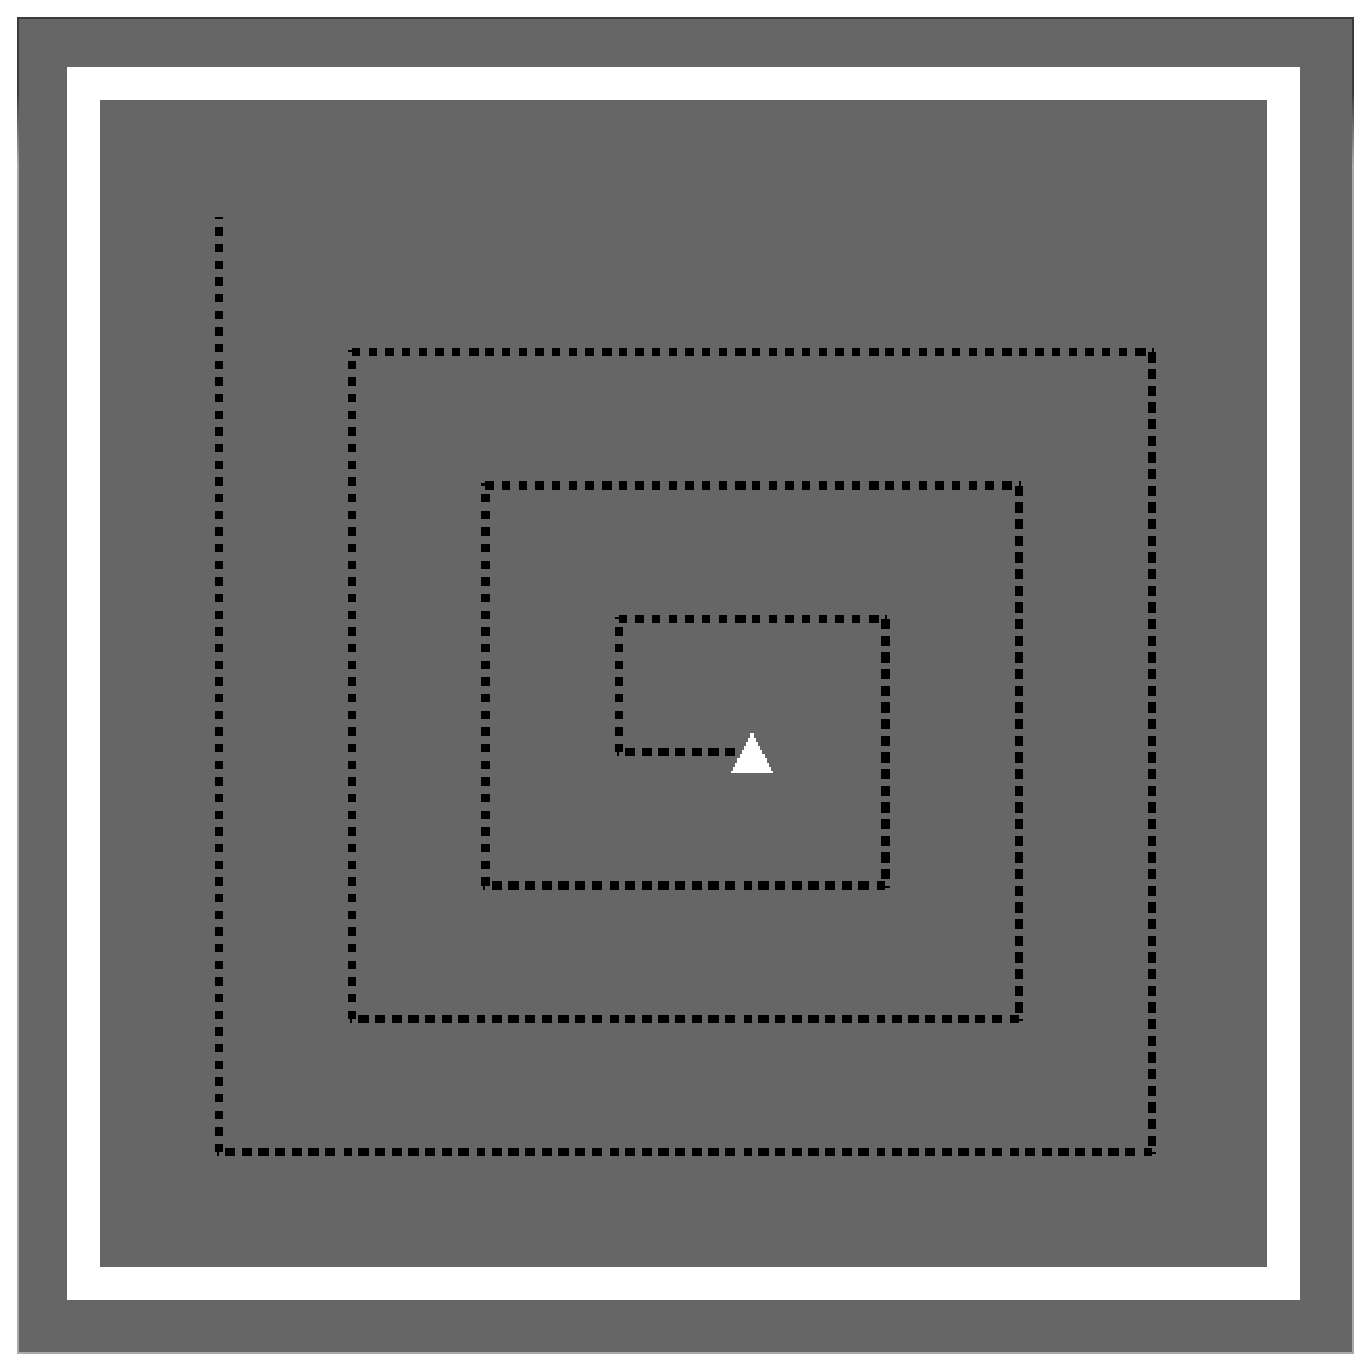
\includegraphics[width=.49\linewidth]{./spiral2}
%\caption{Images generated by our robot simulator using the {\tt spiral} program.An important detail is that the robot simulator does not evaluate the Monadic program but rather executes a compiled first-order representation of that program.}
%\label{fig:spiral}
%\end{figure}


%\begin{figure}
%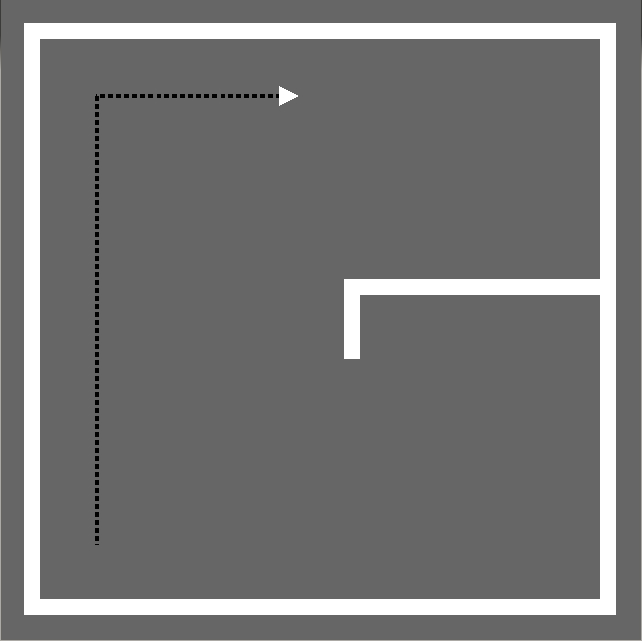
\includegraphics[width=.49\linewidth]{./wall1}
%\includegraphics[width=.49\linewidth]{./wall2}
%\caption{Images generated by the robot simulator using the {\tt followWall} program.}
%\label{fig:followwall}
%\end{figure}


%\FloatBarrier
%Set the mood. \docname{} is more of a deep ``Theory'' kind of person 



%Suppose you have just bought yourself a little programmable toy robot
%and you want to design a small DSL in Haskell to program it. The robot
%can turn, move forward and has a sensor to detect whether it is facing
%an obstacle or not. Inspired by the robot language in \citebb{} you come
%up with a set of primitives shown in figure
%\ref{fig:interface}. In particular, you would like to use the
%do-notation to sequence programs.

%\begin{figure} 
%\begin{itemize} 
%  \item \verb!move      :: Program ()! 
%  \item \verb!turnLeft  :: Program ()!
%  \item \verb!turnRight :: Program ()!
%  \item \verb!sensor    :: Program Bool!
%  \item \verb!cond      :: Program Bool -> Program () -> Program () -> Program ()!
%  \item \verb!while     :: Program Bool -> Program () -> Program ()!
%  \item \verb!instance Monad Program!
%\end{itemize} 
%\label{fig:interface} 
%\caption{Proposed set of basic robot operations} 
%\end{figure}

%\emph{Example programs}


%The next task is to implement this language. Compiling EDSLs like this
%to something which the physical robot can execute is well know and
%there are off-the-shelf techniques to use. But there is one quirk; how
%does one generate an abstract syntax tree from a type which implements
%the Monad interface?

%Since you want to compile the language there must be an abstract
%syntax tree representation of some sort of the language. The natural
%thing is just to create a new type where each language construct has
%its own constructor. But should you deal with the monadic constructs?
%Well, the simplest solution would be to just add them to the type as well. The resulting type 

%\begin{figure}
%\begin{verbatim}
%data BoolE = Lit Bool
%         | Var String
%         | (:||:) BoolE BoolE
%         | (:&&:)  BoolE BoolE
%         | Not BoolE  

%data Program a where
%  Move      :: Program ()
%  TurnRight :: Program ()
%  TurnLeft  :: Program ()

%  Sensor    :: Program BoolE
%  Cond      :: BoolE -> Program () -> Program () -> Program ()
%  While     :: Program BoolE -> Program () -> Program ()
%   
%  Return    :: a -> Program a 
%  Bind      :: Program a -> (a -> Program b) -> Program b
%\end{verbatim}
%\label{fig:program}
%\caption{A data type for programs}
%\end{figure}

%\emph{More text}

%In the rest of this paper we will see that this na\"ive method
%actually can be made to work and that it's a practical, compositional
%technique for reifying monads.
